\section{A finite-time voter closure near the voter point}
\label{sec:theory}

Near $p=1$, write $\varepsilon=1-p$ and $\kappa=q/\varepsilon$, so that
\begin{equation}
 w(j)=\frac j8+\varepsilon g(j),\qquad
 g(j)=\alpha R(j)-\frac j8+\kappa\delta_{j,2}.
 \label{eq:pert}
\end{equation}
Voter-model perturbation theory relates a weak microscopic perturbation to a reaction
term obtained by averaging over voter correlations~\cite{cox2013}. In $d\ge3$ the
required nontrivial voter equilibrium exists. In $d=2$ the voter model clusters and
that stationary reaction function is not defined~\cite{cox2025}. We therefore
separate an exact finite-time calculation from its use as a closure for the
perturbed model.

\subsection{Exact finite-time identities}

Start the unperturbed voter model from independent spins of mean density $u$, and
let $\langle\cdot\rangle_{u,T}$ denote its local law at time $T$. Define
\begin{equation}
 f_T(u)=\big\langle(1-2\sigma_0)g(j_0)\big\rangle_{u,T}.
 \label{eq:f}
\end{equation}
For this specified reference law, $f_T$ is exactly the mean density drift due to
the perturbation, divided by $\varepsilon$. It is not the drift evaluated in the
unknown stationary law of the perturbed process.

The reference expectation can be evaluated by voter duality. Nine coalescing walks
start at the origin and its eight Moore neighbors and run backward for $T$ steps.
For synchronous updating, distinct walks jump independently at each step and
coalesce when their new positions coincide. Each surviving lineage is assigned a
state independently, with probability $u$ of being live. This gives the polynomial
$f_T$ by summing over the lineage partitions and their colorings. We use the
recorded histograms of $10^6$ walk realizations at each cutoff.

Three identities substantially constrain the result. A perturbation linear in
$j$ gives zero drift. One- and two-lineage partitions also give zero by symmetry.
For a three-lineage partition, let $n_1,n_2$ be the numbers of neighbors in the
two classes not containing the origin. Its contribution is
\begin{equation}
 \begin{gathered}
 h(u)\,[g(n_1)+g(n_2)-g(n_1+n_2)],\\
 h(u)=u(1-u)(1-2u).
 \end{gathered}
 \label{eq:three}
\end{equation}
A four-lineage partition contributes the same cubic, with coefficient
$\sum_{i=1}^3g(n_i)-g(\sum_{i=1}^3 n_i)$.
Only partitions with at least five lineages can generate higher-degree terms.
In particular,
\begin{equation}
 f_T=\alpha f_{R,T}+\kappa f_{2,T}
 \label{eq:linearclosure}
\end{equation}
holds exactly at every fixed $T$.

\subsection{Fronts and bistability within the closure}

To use this local calculation for phase selection, we make the additional
approximation
$\partial_tu=D\nabla^2u+\varepsilon f_T(u)$, with a fixed cutoff and constant
diffusion coefficient. The corresponding front criterion is a property of this
deterministic scalar equation, not an exact criterion for the stochastic lattice
process. Put $c=\kappa/\alpha$, and define three closure thresholds:
$c_a(T)$ by $f_T'(0)=0$, $c_h(T)$ by $f_T'(1/2)=0$, and $c_f(T)$ by
$\int_0^{1/2}f_T(u)\,\ds u=0$. The last condition gives a stationary front when
both endpoint states are stable~\cite{durrett1994b,durrett2009}. All three
thresholds have the fixed-cutoff form
\begin{equation}
 q_x(T)=\alpha(1-p)c_x(T),\qquad x\in\{a,h,f\}.
 \label{eq:line}
\end{equation}
The linear dependence is exact within the closure at a specified cutoff;
identifying $q_f(T)$ with the physical $\qs$ requires a matching prescription.

The role of the higher-lineage terms can be made explicit without fitting a
polynomial shape. For $X\in\{R,2\}$ write
\[
 \begin{gathered}
 A_X=f_{X,T}'(0),\qquad
 I_X=\int_0^{1/2}f_{X,T}(u)\,\ds u,\\
 B_X=I_X-A_X/32.
 \end{gathered}
\]
Since $\int_0^{1/2}h(u)\,\ds u=1/32$, $B_X$ receives contributions only from
partitions with at least five lineages. Provided the denominators are nonzero,
\begin{equation}
 c_a-c_f=
 \frac{32(A_2B_R-A_RB_2)}{A_2(A_2+32B_2)}.
 \label{eq:lineagesplitting}
\end{equation}
Deleting the higher-lineage partitions makes this splitting exactly zero.
Their presence is necessary, although their sign and weight still decide whether
the full reaction term is bistable.

For the D\&N perturbation the sampled closures satisfy $c_h<c_f<c_a$, with both
endpoint states stable and one unstable root in $0<u<1/2$ at $c_f$.
The finite-cutoff splitting is well resolved:
\begin{center}
\begin{tabular}{rccc}
$T$ & $c_h$ & $c_f$ & $c_a-c_f$\\
\hline
64 & $0.17770(73)$ & $0.23142(70)$ & $0.12395(38)$\\
1024 & $0.22941(119)$ & $0.24843(119)$ & $0.04008(29)$\\
65536 & $0.25036(191)$ & $0.25526(191)$ & $0.00994(21)$
\end{tabular}
\end{center}
Parentheses here give one standard error from walk sampling only. They do not
include the uncertainty of the closure or its cutoff. The errors of $c_a$ and
$c_f$ are strongly correlated: their correlation is $0.994$ at $T=65536$.
Consequently the uncertainty of their difference is much smaller than either
individual uncertainty. A multinomial bootstrap preserving this correlation
gives a $95\%$ interval approximately $[0.00955,0.01035]$ for $c_a-c_f$ there.
The decreasing window is a property of the finite-time reaction closures.

\begin{figure*}
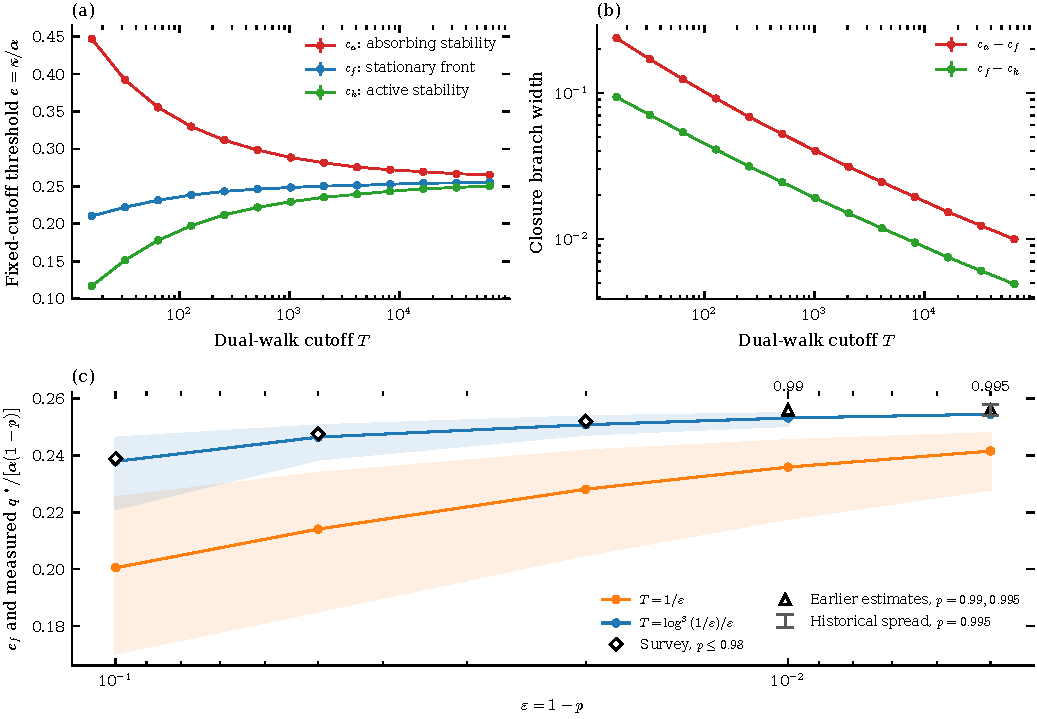
\includegraphics[width=\textwidth]{figs/fig_theory_v2}
\caption{Finite-time voter closure and cutoff sensitivity.
(a) Absorbing-state, stationary-front, and active-state thresholds of the
constant-diffusion closure at cutoff $T$. Bars are approximately 95\%
pointwise intervals from walk sampling.
(b) The two branches of the closure's bistable interval, with covariance
between thresholds retained.
(c) Matching prescriptions $T=1/\varepsilon$ and
$T=\log^3(1/\varepsilon)/\varepsilon$ compared with the finite-window
survey. Open triangles mark the earlier $p=0.99$ and 0.995 estimates.
The $p=0.995$ whisker is the historical spread
$q=0.000640\pm0.000005$, equivalent to $c=0.256\pm0.002$;
it represents estimator sensitivity. The longer $2\times10^7$-step runs
at that probability continue to decay. Shading varies either prescribed
time by a factor $A\in[1/4,4]$. The shading and historical whisker have
no assigned confidence coverage. Interpolation uses only recorded
cutoffs, leaving the upper logarithmic envelope incomplete at the
smallest $\varepsilon$.}
\label{fig:theory}
\end{figure*}

\subsection{Matching uncertainty and the voter endpoint}

In two dimensions the probability of retaining several distinct voter lineages
decays logarithmically with time~\cite{cox2010,cox2025}. The scale on which a
perturbation acts can therefore differ from $1/\varepsilon$ by logarithmic
factors. For example, the two-dimensional scaling of Ref.~\cite{cox2025}
uses $\varepsilon_N=(\log N)^3/N$. That result does not derive a matching
time for the present synchronous automaton, especially close to cancellation
of its leading cubic drift, but it motivates checking sensitivity to such
factors.

Figure~\ref{fig:theory}(c) compares the unadjusted prescriptions
$T=1/\varepsilon$ and $T=\log^3(1/\varepsilon)/\varepsilon$:
\begin{center}
\begin{tabular}{cccc}
$p$ & measured $c$ & $c_f(1/\varepsilon)$ & $c_f(\log^3(1/\varepsilon)/\varepsilon)$\\
\hline
0.9 & 0.2388 & 0.2005 & 0.2379\\
0.95 & 0.2476 & 0.2141 & 0.2464\\
0.98 & 0.2520 & 0.2281 & 0.2507\\
0.99 & 0.2560 & 0.2359 & 0.2531\\
0.995 & 0.2560 & 0.2415 & 0.2545
\end{tabular}
\end{center}
The logarithmic prescription substantially improves this comparison without
adjusting its prefactor. This comparison is sensitive to the matching scale, but does not validate
the prescription. In particular, the historical spread $5\times10^{-6}$ in
$q^*$ at $p=0.995$ corresponds to about $0.002$ in $c$, larger than the
theory--central-value difference at that point. That historical density
plateau subsequently decays (Fig.~\ref{fig:gpu_near20m}).
Multiplying either prescribed time by $A=1/4,1,4$ displays the remaining
sensitivity. Interpolation is linear in $\log T$; points beyond the recorded
range are left unevaluated.

The walk statistics constrain the closure much more precisely than they fix
its relation to the lattice process. For example, over $1024\le T\le65536$,
$c_f$ moves from $0.24843$ to $0.25526$, while its one-standard-error sampling
uncertainty grows from $0.00119$ to $0.00191$. We therefore do not assign a
confidence interval to a $T\to\infty$ amplitude. The same walks contribute
to successive checkpoint histograms; the stored marginal counts do not
recover their cross-time covariance, and we do not treat those checkpoints
as independent observations in an extrapolation.

The lazy-walk calculation gives another independent test of the closure.
At physical dual time $rT=65536$, it gives $c_f=0.2212$, $0.2060$, and
$0.2003$ for $r=1/2,1/4,1/8$, respectively, compared with measured values
about $0.218,0.216,0.219$. It captures the initial direction of the shift.
The measured differences among the smaller $r$ values lie below the
front-fit systematic variation discussed in Sec.~\ref{S-sec:async}, so this
comparison does not resolve a limiting amplitude. The five-cell rule in
Supplemental Sec.~\ref{S-app:molofsky} supplies a sharper limitation: no single cutoff describes its early seed-growth crossover, observed bulk
stationarity range, and extrapolated onset of coherent expansion.

The exact identities identify a mechanism available to a voter perturbation:
higher-lineage correlations generate the noncubic drift needed for a bistable
reaction term. They also explain why that contribution becomes small at long
voter times within the closure. Whether it remains effective after matching
and fluctuation corrections is not determined by the calculation. Persistence
of a first-order line for every fixed $p<1$, and its logarithmic approach to
the voter point, remain conjectures; the numerical evidence for finite $p$
is assessed separately in Sec.~\ref{sec:voter}.

